\documentclass[10pt, a4paper]{article}
\usepackage{float} % display graphics at the demanded place
\usepackage{hyperref} % display table des matières
\usepackage{subcaption} % authorize subfigure
\usepackage{booktabs}
\usepackage[utf8]{inputenc}
\usepackage[T1]{fontenc}
%\usepackage[french]{babel} %casse tout chez moi
\usepackage{graphicx}

%élargi un peu pour que les diagrammes soient pas minuscules ou mal alignés
\evensidemargin=0in
\oddsidemargin=0in
\textwidth=6.5in

\graphicspath{{Diagrammes/}}


\title{INFO-F-109 : Projet d'informatique 2 \\
       \textbf{Software requirement document\\
	   Pawn Hub}}
\author{Huward Maxence, Boonen Jacques\\
		Pham Hong Phuc, Duc Nguyen, Caroline Forest\\
		Antunes Andre, Romain Mardulyn}
\date{17 Décembre 2018}
\begin{document}
	\maketitle
	\tableofcontents %do a table of content automatically	
	\newpage
	\section{Introduction}
		\subsection{Description du projet}
			\paragraph{}L'objectif de ce projet est de recréer un grand classique des jeux de plateau: les échecs. Le but est d'implémenter une plateforme multijoueurs permettant de jouer en ligne le jeu classique ainsi que ses variantes.
Les joueurs auront des comptes utilisateurs et pourront intéragir entre eux sur la plateforme.
En plus du jeu usuel 8x8, nous allons aussi inclure les variantes de : AliceChess, DarkChess et HordeChess.

		\subsection{Historique des modifications}
		
		\begin{table}[h!]
			\centering
			\begin{tabular}{|c|c|c|p{50mm}|}
				\hline
				 \textbf{version} & \textbf{date} & \textbf{auteur}  & \textbf{description} \\ \hline
				 1 & 4/12 & Pham Hong Phuc & Création du SRD en LaTex\\ \hline
				 1.1 & 6/12 & Caroline Forest & Ajout de diagrammes UML\\ \hline

\end{tabular}
			\caption*{Historique des modifications}
			\end{table}
%fin du tableau

%BESOINS UTILISATEURS%

	\section{Besoins utilisateurs}
		\subsection{Fonctionnels}
		
%pas sure qu'on le garde, ou le mettre, tout ca.
%Je pense que le main menu est mieux finalement
\begin{figure}[ht]
\centering
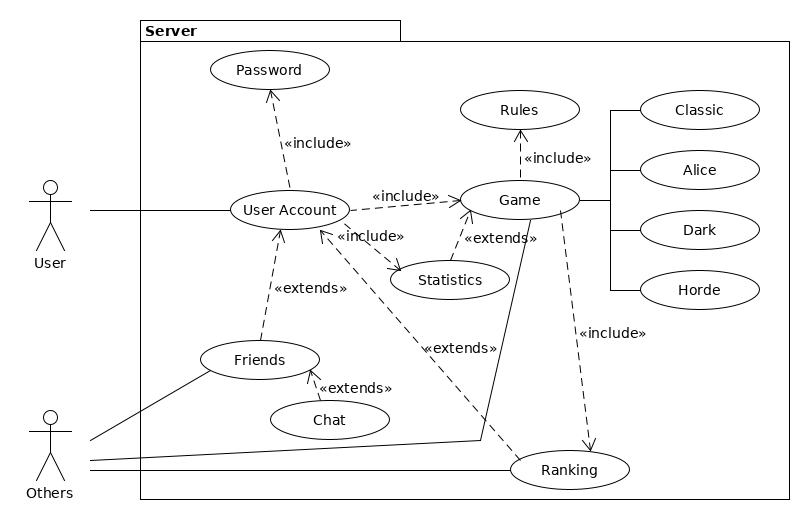
\includegraphics[scale=0.4]{UC_useractions.png}
\caption{Diagramme de \textit{use case} des actions possibles d'un utilisateur}
\label{UC_act} %UseCase_actions
\end{figure}

\begin{figure}[ht]
\centering
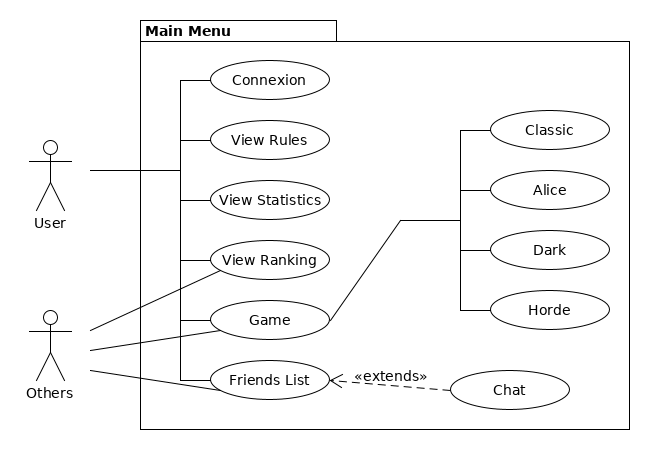
\includegraphics[scale=0.4]{UC_mainmenu.png}
\caption{Diagramme de \textit{use case} des actions possibles d'un utilisateur}
\label{UC_menu} %UseCase_menu
\end{figure}

\subsubsection{Connection}
Sera détaillé en \ref{connexion}.

\subsubsection{Voir les Règles}
\textbf{Acteur :} \textit{User}.\\
\textbf{Relations avec d'autres cas d'utilisation :} Néant.\\
\textbf{Pré-conditions :} Le \textit{user} doit avoir sélectionné l'option \textit{View Rules} dans le menu principal du jeu.\\
\textbf{Post-conditions :} Le \textit{user} accède aux règles de jeu.\\
\textbf{Cas général :} Le \textit{user} peut consulter les règles de jeu en envoyant une requête au serveur.\\
\textbf{Cas exceptionnels :} Néant.

\subsubsection{Voir les Statistiques Personnelles}
\textbf{Acteur :} \textit{User}.\\
\textbf{Relations avec d'autres cas d'utilisation :} Néant.\\
\textbf{Pré-conditions :} Le \textit{user} doit avoir sélectionné l'option \textit{View Statistics} dans le menu principal du jeu.\\
\textbf{Post-conditions :} Le \textit{user} accède à ses statistiques personnelles.\\
\textbf{Cas général :} Le \textit{user} peut consulter ses statistiques en envoyant une requête au serveur.\\
\textbf{Cas exceptionnels :} Néant.

\subsubsection{Voir le Classement}

\textbf{Acteur :} \textit{User}.\\
\textbf{Relations avec d'autres cas d'utilisation :} Néant.\\
\textbf{Pré-conditions :} Le \textit{user} doit avoir sélectionné l'option \textit{View Ranking} dans le menu principal du jeu.\\
\textbf{Post-conditions :} Le \textit{user} accède au classement global des joueurs (\textit{user} et \textit{others}).\\
\textbf{Cas général :} Le \textit{user} peut consulter le classement global des joueurs (\textit{user} et \textit{others}) en envoyant une requête au serveur.\\
\textbf{Cas exceptionnels :} Néant.

\subsubsection{Jouer}

\textbf{Acteur :} \textit{User}.\\
\textbf{Relations avec d'autres cas d'utilisation :} Modes de jeu proposés (\textit{Classic},\textit{Alice}, \textit{Dark} ou \textit{Horde}).\\
\textbf{Pré-conditions :} Le \textit{user} doit avoir sélectionné l'option \textit{Game} dans le menu principal du jeu.\\
\textbf{Post-conditions :} Le \textit{user} selectionne un mode de jeu parmi ceux proposés(\textit{Classic},\textit{Alice}, \textit{Dark} ou \textit{Horde}).\\
\textbf{Cas général :} Le \textit{user} peut sélectionner un mode de jeu parmi ceux proposés(\textit{Classic},\textit{Alice}, \textit{Dark} ou \textit{Horde}), ce qui lance une requête de \textit{matchmaking} (voir \ref{matchmaker}) au serveur.\\
\textbf{Cas exceptionnels :} Néant.

\subsubsection{Liste d'Amis}

\textbf{Acteur :} \textit{User}.\\
\textbf{Relations avec d'autres cas d'utilisation :} \textit{Chat}.\\
\textbf{Pré-conditions :} Le \textit{user} doit avoir sélectionné l'option \textit{Liste d'Amis} dans le menu principal du jeu.\\
\textbf{Post-conditions :} Le \textit{user} accède à sa liste d'utilisateurs 'amis', avec lesquels il peut choisir de discuter, via l'option \textit{chat}.\\
\textbf{Cas général :} Le \textit{user} peut consulter sa liste d'utilisateurs 'amis' en envoyant une requête au serveur. Il peut aussi discuter avec eux via messages instantanés et le serveur.\\
\textbf{Cas exceptionnels :} Néant.
		
		\subsection{Connection}
\label{connexion}
\begin{figure}[h]
\centering
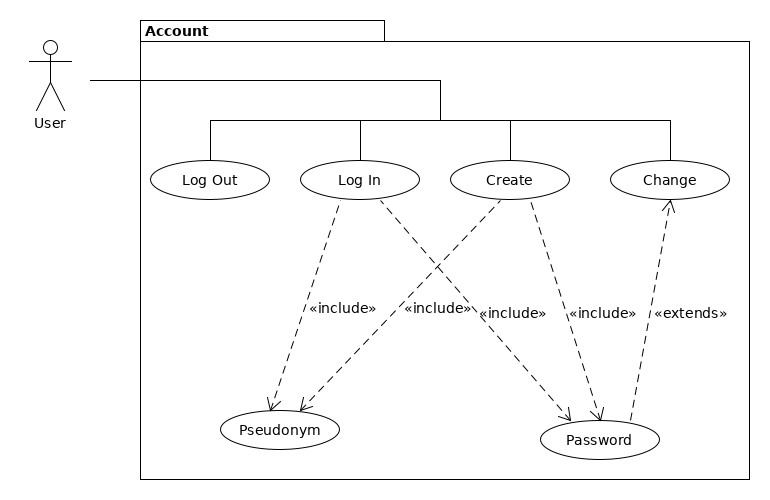
\includegraphics[scale=0.4]{UC_connexion.png}
\caption{Diagramme de \textit{use case} de connexion d'un utilisateur}
\label{UC_co} %UseCase_connection
\end{figure}

		\subsection{Durant une partie}
		
		\subsection{Non-fonctionnels}
		
	\section{Besoins systèmes}
		\subsection{Fonctionnels}
		\subsubsection{Connexion au serveur}
		
		\subsubsection{Partie joueur vs. joueur}
		\label{matchmaker}
		
\begin{figure}[ht]
\centering
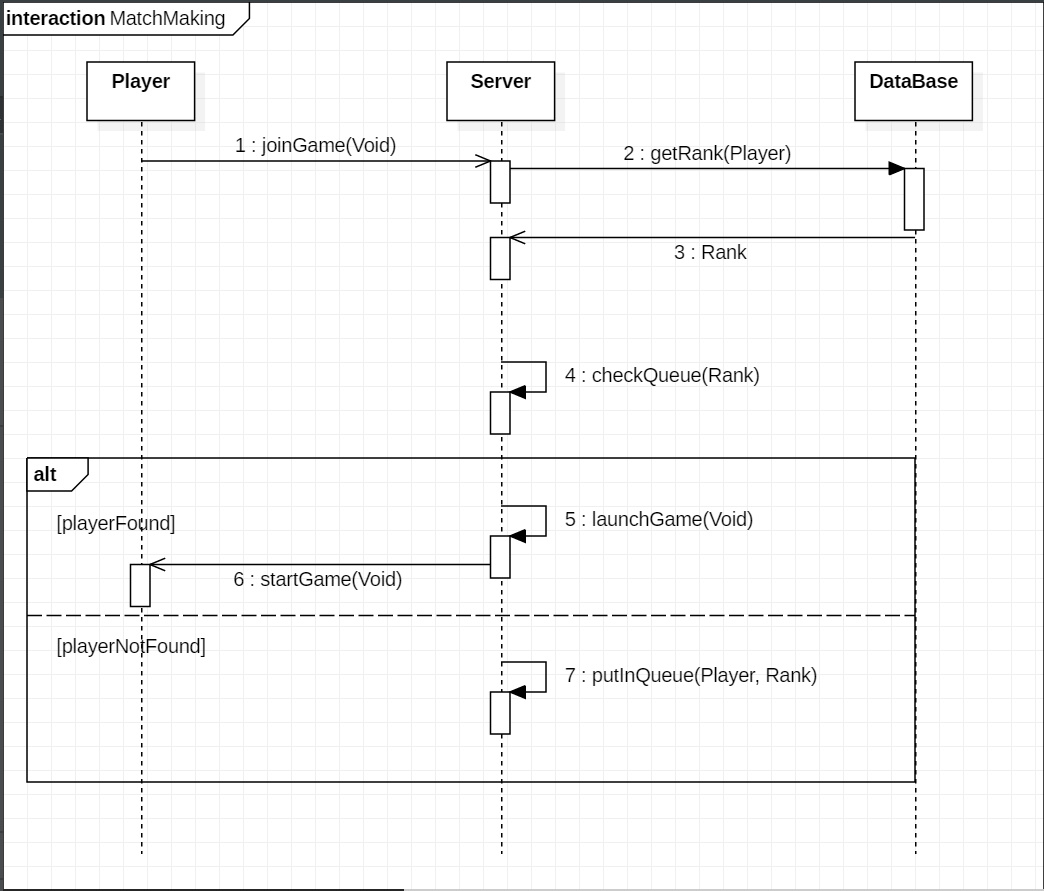
\includegraphics[scale=0.45]{SequenceDiagramMatchmaking.PNG}
\caption{Diagramme de séquence pour le \textit{Matchmaking}}
\label{SD_matchmaker} %SequenceDiagram_matchmaking
\end{figure}

		\label{classicgame}
\begin{figure}[ht]
\centering
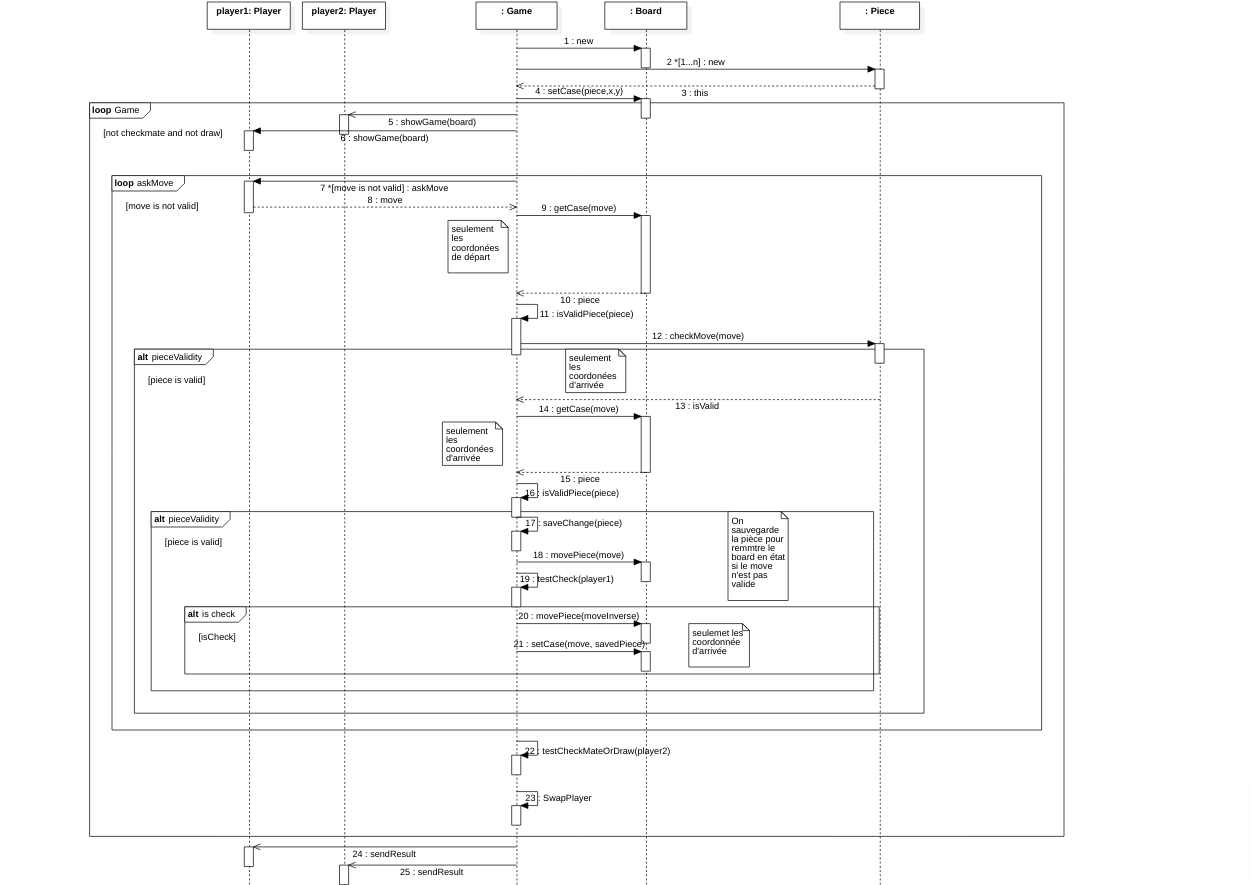
\includegraphics[scale=0.45]{SequenceDiagramClassicChessTurn.png}
\caption{Diagramme de séquence pour le fonctionnement d'une partie}
\label{SD_classicgame} %SequenceDiagram_classicgame
\end{figure}
\clearpage
		
		\subsection{Non-fonctionnel}
		
	\section{Design du système}
	
\begin{figure}[ht]
\centering
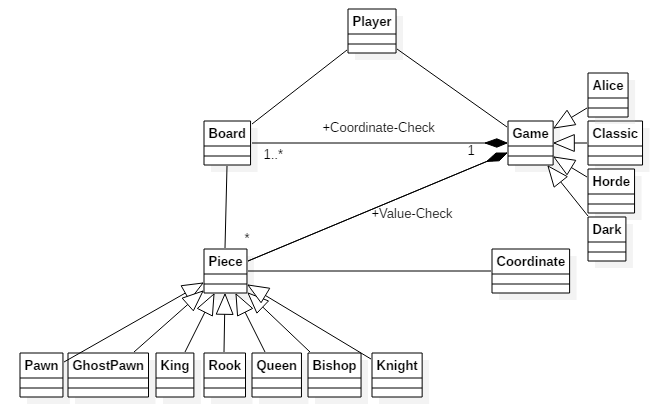
\includegraphics[scale=0.4]{ClassDiagram.png}
\caption{Diagramme de classes général}
\label{CD} %ClassDiagram
\end{figure}
		
		\subsection{Connexion du joueur}
		
		\subsection{Les actions du joueur}
		
		\subsection{Client-Serveur}
		\paragraph{}Le serveur aura une copie du board et se tâchera de devoir vérifier les différentes actions des joueurs. Il veillera également à  mettre à jour les board des joueurs.
		\subsection{Les modes de jeu}
		\paragraph{}Quatre modes sont proposés:
		
		\subsection{Menu}
		
	\section{Annexe}
	
	
		
		
		
		

\end{document}